%
\documentclass[10pt]{standalone}
\input{../../tikzpic_packages.tex}

\begin{document}

%
%Bein 2 - Anheben und Fallen lassen.
%\begin{tabular}{ll}
%
%2 & 0\\
%5 & 0\\
%10 & .14\\
%15 & .19\\
%20 & .25\\
%25 & .32\\
%30 & .38\\
%35 & .42\\
%40 & .49\\
%45 & .51\\
%50 & .53\\
%55 & .57\\
%60 & .60\\
%65 & .62\\
%70 & .64\\
%75 & .65\\
%80 & .67\\
%85 & .69\\
%88 & .7\\
%\end{tabular}
%
%
%
%
%
%
%
%Bein 2 - Gleiten auf Ebene 0$^\circ$.
%\begin{tabular}{ll}
%
%2 & 0\\
%5 & 0.24\\
%10 & .32\\
%15 & .38\\
%20 & .42\\
%25 & .47\\
%30 & .52\\
%35 & .55\\
%40 & .58\\
%45 & .61\\
%50 & .63\\
%55 & .65\\
%60 & .67\\
%65 & .68\\
%70 & .70\\
%75 & .71\\
%80 & .73\\
%85 & .74\\
%88 & .75\\
%85 & .63\\
%80 & .60\\
%75 & .57\\
%70 & .53\\
%65 & .49\\
%60 & .46\\
%55 & .42\\
%50 & .36\\
%45 & .30\\
%40 & .23\\
%35 & .15\\
%30 & .08\\
%25 & .00\\
%20 & .\\
%15 & .\\
%10 & .\\
%5 & .\\
%2 & .\\
%\end{tabular}
%
%
%
%
%
%Bein 1 - Anheben und Fallen lassen.
%\begin{tabular}{ll}
%
%2 & 0\\
%5 & 0\\
%10 & .08\\
%15 & .19\\
%20 & .29\\
%25 & .37\\
%30 & .42\\
%35 & .48\\
%40 & .53\\
%45 & .56\\
%50 & .61\\
%55 & .64\\
%60 & .67\\
%65 & .69\\
%70 & .71\\
%75 & .72\\
%80 & .73\\
%85 & .75\\
%88 & .76\\
%\end{tabular}
%
%
%
%Bein 1 - Gleiten auf Ebene 0$^\circ$.
%\begin{tabular}{ll}
%
%2 & 0\\
%5 & 0.20\\
%10 & .33\\
%15 & .40\\
%20 & .48\\
%25 & .53\\
%30 & .58\\
%35 & .63\\
%40 & .67\\
%45 & .71\\
%50 & .74\\
%55 & .77\\
%60 & .79\\
%65 & .81\\
%70 & .83\\
%75 & .84\\
%80 & .85\\
%85 & .855\\
%88 & .89\\
%85 & .71\\
%80 & .68\\
%75 & .62\\
%70 & .57\\
%65 & .52\\
%60 & .47\\
%55 & .42\\
%50 & .37\\
%45 & .30\\
%40 & .23\\
%35 & .16\\
%30 & .07\\
%25 & .00\\
%20 & .\\
%15 & .\\
%10 & .\\
%5 & .\\
%2 & .\\
%\end{tabular}
%


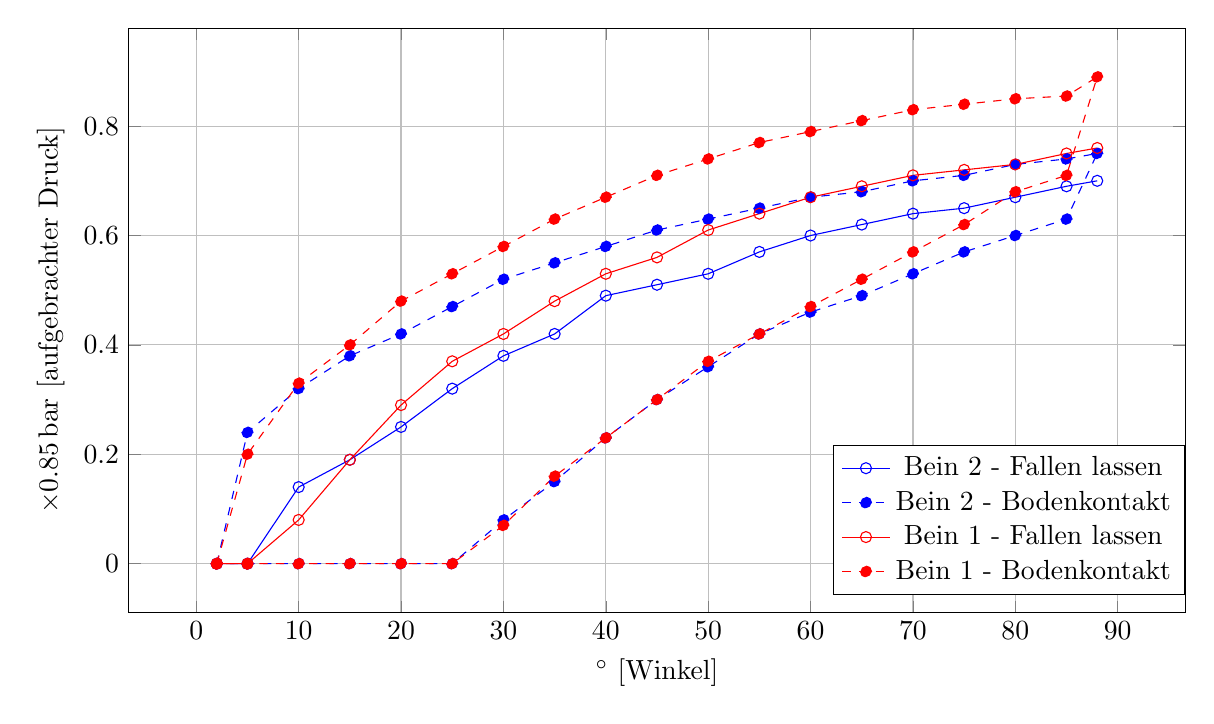
\begin{tikzpicture}
	\begin{axis}[
		height=9cm,
		width=15cm,
		grid=major,
		legend style={at={(1,0.03)},anchor=south east},
		xlabel={$^\circ$ [Winkel]},
		ylabel={$\times 0.85$\,bar [aufgebrachter Druck]}
	]
	\addplot[solid, mark=o, blue] coordinates {
		(2 , 0)(5 , 0)(10 , .14)(15 , .19)(20 , .25)(25 , .32)(30 , .38)(35 , .42)(40 , .49)(45 , .51)(50 , .53)(55 , .57)(60 , .60)(65 , .62)(70,.64)(75 , .65)(80 , .67)(85 , .69)(88 , .7)
	};
	\addlegendentry{Bein 2 - Fallen lassen}
	
	
	\addplot[dashed, mark=*, blue] coordinates{
		(2,0)(5,0.24)(10,.32)(15,.38)(20,.42)(25,.47)(30,.52)(35,.55)(40,.58)(45,.61)(50,.63)(55,.65)(60,.67)(65,.68)(70,.70)(75,.71)(80,.73)(85,.74)(88,.75)(85,.63)(80,.60)(75,.57)(70,.53)(65,.49)(60,.46)(55,.42)(50,.36)(45,.30)(40,.23)(35,.15)(30,.08)(25,.00)(20,.)(15,.)(10,.)(5,.)(2,.)
	};
	\addlegendentry{Bein 2 - Bodenkontakt}

	\addplot[solid, mark=o, red] coordinates{
		(2,0)(5,0)(10,.08)(15,.19)(20,.29)(25,.37)(30,.42)(35,.48)(40,.53)(45,.56)(50,.61)(55,.64)(60,.67)(65,.69)(70,.71)(75,.72)(80,.73)(85,.75)(88,.76)
	};
	\addlegendentry{Bein 1 - Fallen lassen}

	\addplot[dashed, mark=*, red] coordinates{
		(2,0)(5,0.20)(10,.33)(15,.40)(20,.48)(25,.53)(30,.58)(35,.63)(40,.67)(45,.71)(50,.74)(55,.77)(60,.79)(65,.81)(70,.83)(75,.84)(80,.85)(85,.855)(88,.89)(85,.71)(80,.68)(75,.62)(70,.57)(65,.52)(60,.47)(55,.42)(50,.37)(45,.30)(40,.23)(35,.16)(30,.07)(25,.00)(20,.)(15,.)(10,.)(5,.)(2,.)
	};
	\addlegendentry{Bein 1 - Bodenkontakt}	

	\end{axis}
\end{tikzpicture}

\end{document}
